\documentclass[a4paper, 12pt]{article}
\usepackage[utf8]{inputenc}  % Unicode
\usepackage[french]{babel}
\usepackage{geometry}
\usepackage{graphics}
\usepackage[pdftex]{graphicx, color}
\usepackage{pdfpages}
\DeclareGraphicsExtensions{.jpg,.png}
\pdfoutput=1
\usepackage[pdftex,
	bookmarks = true,           % Signets
	bookmarksnumbered = true,   % Signets numerotes
	pdfstartview = FitV,        % La page prend toute la hauteur
	colorlinks=true,
	citecolor=black,urlcolor=blue,linkcolor=black,
	pdfauthor={Auteur},
	pdftitle={Titre},
 	pdfsubject={Sujet},
%	pdfkeywords={},	% Besoin de keywords ?
	plainpages=false,
	pdfpagelabels,
	breaklinks=true,
   	hyperindex,
	linktocpage=true	% pour colorier seulement le numéros dans la TOC	
]{hyperref}
\usepackage{float}
\usepackage{listings}
\usepackage{alltt}
\usepackage{amsmath}
\renewcommand{\ttdefault}{txtt}

\lstset{basicstyle=\ttfamily,
escapeinside={||},
mathescape=true}
\setcounter{secnumdepth}{3}
\newcommand{\HRule}{\rule{\linewidth}{0.5mm}}

\newcommand*\styleC{\fontsize{9}{10pt}\selectfont }
\newcommand*\styleD{\fontsize{9}{10pt}\usefont{OT1}{pag}{m}{n}\selectfont }

\makeatletter
% on fixe le langage utilisé
\lstset{language=matlab}
\edef\Motscle{emph={\lst@keywords}}
\expandafter\lstset\expandafter{
}
\makeatother



\definecolor{Ggris}{rgb}{0.45,0.48,0.45}

\lstset{emphstyle=\ttfamily\color{blue}, % les mots réservés de matlab en bleu
basicstyle=\ttfamily\styleC, % 
keywordstyle=\ttfamily,
commentstyle=\color{Ggris}\styleD, % \styleD commentaire en gris
numberstyle=\tiny\color{black},
numbers=left,
numbersep=10pt,
lineskip=0.7pt,
showstringspaces=false}
%  % inclure le fichier source
\newcommand{\FSource}[1]{%
\lstinputlisting[texcl=true]{#1}
}

%%%%%%%%%
\textwidth=15cm
\textheight=21cm
%\hoffset=-2.5cm
\tolerance=9000
\hbadness=9000
\pretolerance=2500


\begin{document}
%\rmfamily

\begin{titlepage}
\begin{center}



\textsc{\Large Rapport de TP - SY26}\\[0.5cm]
\vspace{4cm}
% Title
\HRule \\[0.4cm]
{ \huge \bfseries TP02 - Codage de Huffman \\[0.4cm] }

\HRule \\[1.5cm]

% Author and supervisor
\begin{minipage}{0.4\textwidth}
\begin{flushleft} \large
R\'emi \textsc{Burtin}
\end{flushleft}
\end{minipage}
\begin{minipage}{0.4\textwidth}
\begin{flushright} \large
Cyril \textsc{Fougeray}
\end{flushright}
\end{minipage}

\vspace{4cm}

{\large \today}



\vfill
% Bottom

\includegraphics[width=0.25\textwidth]{logo.jpg}\\[0.5cm]

\textsc{\LARGE Universit\'{e} de Technologie de Compi\`{e}gne}\\[1.5cm]


\end{center}
\end{titlepage}


%\begin{abstract} 
%\end{abstract} 

%{\bf Keywords:} \newline


\clearpage

\section{Introduction}

Le but de ce TP est de mettre en œuvre certaines étapes de l’algorithme de compression JPEG.

\section{Transformée en cosinus discrète (DCT)}

\subsection{Mise en œuvre de la fonction MyDCT}\label{}

Cette première fonction nous permet de calculer la transformée en cosinus discrète d'un bloc de taille 8x8.

Pour cela, nous utilisons les formules suivantes :\\

$D = X_mBY_m^T$ \\ 

avec $X_m(u,x) = \frac{1}{2}C(u) cos(\frac{(2x + 1)\pi u }{16})$ et $Y_m(v,y) = \frac{1}{2}C(v) cos(\frac{(2x + 1)\pi v }{16})$ \\

en prenant $C(0) = \frac{1}{\sqrt{2}}$ et $C(k)=1$ pour $k \in [1..7]$. \\

Les coefficient $u$ et $v$ varie de 0 à 7, donc les matrices $X_m$ et $Y_m$ ont 8 lignes. Par ailleurs, la matrice $B$ avec laquelle nous travaillons est une matrice 8x8. Ainsi, les coefficients $x$ et $y$ sont pris entre 1 et 8. On obtient donc $X_m = Y_m$. \\

Nous calculons les matrices $X_m$ et $Y_m$ en remplaçant les 4 variables $(u, v, x, y)$ dans les formules, nous multiplions les matrices $X_m$, $B$ et $Y_m$ et obtenons ainsi la matrice $D$, la transformée en cosinus discrète de $B$.\\

Le code de la fonction est en annexe \ref{dct_code}.

\subsubsection{R\'esultats}
\label{sec:Resultats}

Après avoir exécuté la fonction, nous nous rendons compte du résultat : 

\begin{alltt}
>> Bref=[	139 144 149 153 155 155 155 155;
					144 151 153 156 159 156 156 156;
					150 155 160 163 158 156 156 156;
					159 161 162 160 160 159 159 159;
					159 160 161 162 162 155 155 155;
					161 161 161 161 160 157 157 157;
					162 162 161 163 162 157 157 157;
					162 162 161 161 163 158 158 158];

>> BrefDCT = MyDCT(Bref)

BrefDCT =

   1.0e+03 *

 1.2596   -0.0010   -0.0121   -0.0052    0.0021   -0.0017   -0.0027    0.0013
-0.0226   -0.0175   -0.0062   -0.0032   -0.0029   -0.0001    0.0004   -0.0012
-0.0109   -0.0093   -0.0016    0.0015    0.0002   -0.0009   -0.0006   -0.0001
-0.0071   -0.0019    0.0002    0.0015    0.0009   -0.0001   -0.0000    0.0003
-0.0006   -0.0008    0.0015    0.0016   -0.0001   -0.0007    0.0006    0.0013
 0.0018   -0.0002    0.0016   -0.0003   -0.0008    0.0015    0.0010   -0.0010
-0.0013   -0.0004   -0.0003   -0.0015   -0.0005    0.0017    0.0011   -0.0008
-0.0026    0.0016   -0.0038   -0.0018    0.0019    0.0012   -0.0006   -0.0004
\end{alltt}

La matrice $BrefDCT$ correspond au résultat souhaité. \\



\section{Quantification}

Cette partie nous permet de calculer une matrice de quantification, qui nous permettra ensuite de quantifier le bloc après la DCT. Le bloc quantifié s'obtient en divisant chacun des coefficients après la transformée en cosinus discrète par le facteur de quantification situé à la même position dans la matrice de quantification $QM$ :
	\[ Dq(i,j) = \left\lfloor \frac{D(i,j)}{QM(i,j)} + 0.5 \right\rfloor
	\]
	

L'oeil humain étant sensible aux fréquences basses (situées dans le coin supérieur gauche de la matrice après DCT), nous devons diviser ces coefficients par un facteur faible. Voici la matrice utilisée pour un facteur $\textit{Quality} = 50$ :  \\

$QM = \begin{bmatrix}
	16 & 11 & 10 & 16 & 24  & 40  & 51  & 61  \\
	12 & 12 & 14 & 19 & 26  & 58  & 60  & 55  \\
	14 & 13 & 16 & 24 & 40  & 57  & 69  & 56  \\
	14 & 17 & 22 & 29 & 51  & 87  & 80  & 62  \\
	18 & 22 & 37 & 56 & 68  & 109 & 103 & 77  \\
	24 & 35 & 55 & 64 & 81  & 104 & 113 & 92  \\
	49 & 64 & 78 & 87 & 103 & 121 & 120 & 101 \\
	72 & 92 & 95 & 98 & 112 & 100 & 103 & 99
\end{bmatrix} * Fq$


Le facteur \textit{Quality} fourni à la fonction en paramètre d’entrée est compris entre 1 (très mauvais) et 100
(très bien). Si $Quality = 50$ alors $Fq = 1$. Afin de trouver la fonction $f()$ prenant comme paramètre \textit{Quality}, nous avons recherché du côté des standards JPEG qui nous dit :


\[ Fq(Quality) = \left\{ 
  \begin{array}{l l}
    (100 - Quality)/50 & \quad \text{$Quality \geq 50$}\\
    50/Quality & \quad \text{sinon}
  \end{array} \right.\]

Nous obtenons ainsi $Fq$. La matrice de quantification est alors modifiée en conséquence. Il faut faire attention à ce que les valeurs de la matrice soit compris entre 1 et 255. Si certaines valeurs sont plus petites (\textit{resp.} plus grandes) nous les fixons à 1 (\textit{resp.} à 255). Pour cela, nous utilisons la fonction \textit{find}, cf Annexe \ref{quant_code}.\\

Nous avons maintenant la matrice de quantification, nous pouvons alors calculer $Dq$, le bloc quantifié après la DCT : 
\begin{alltt}
Dq = round(BrefDCT./QM)
\end{alltt}


\section{Parcours en zigzag}

Afin de pouvoir compresser efficacement l’information du bloc \textit{Dq}, on se propose de transformer la matrice 8x8 en un vecteur de longueur 64 en parcourant le bloc dans un ordre qui favorise la concentration des coefficients nuls à la fin du vecteur.\\

\begin{figure}[h]
	\centering
		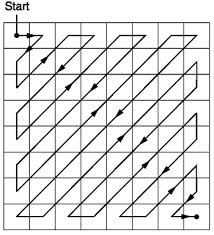
\includegraphics[scale=0.5]{zigzag.jpg}
	\label{fig:zigzag}
\end{figure}


Pour cela, nous avons à disposition un vecteur contenant les indexes des positions successives du parcours en zigzag dans le bloc 8x8. Matlab nous permet facilement de récupérer le vecteur à partir ce des indexes. En effet, prenons cet exemple simple : 

\begin{alltt}
>> a = [5 4 3 2 1]
a =
     5     4     3     2     1

>> a([1 3 5])
ans =
     5     3     1
\end{alltt}

Nous voyons que pour récupérer les valeurs d'un vecteur à des indexes précis, nous pouvons passer en paramètre du vecteur un vecteur d'indexes. Nous faisons de même pour le parcours en zigzag dans un bloc 8x8 :

\begin{alltt}
%% Le parcours en ZigZag (Indexes)
zig=[1 9 2 3 10 17 25 18 ...
     11 4 5 12 19 26 33 41 ...
     34 27 20 13 6 7 14 21 ...
     28 35 42 49 57 50 43 36 ...
     29 22 15 8 16 23 40 37 ...
     44 51 58 59 52 45 38 41 ...
     24 32 38 46 53 60 61 54 ...
     47 40 48 55 62 63 56 64];

Vzig=Dq(zig);
\end{alltt}


\section{Codage}

Pour le codage du bloc, nous appliquons l'algorithme RLE (Run-Length-Encoding). Nous avons vu que le nombre de zéros dans un bloc après DCT est important (tant que l'image a des fréquences relativement basses) et que seul le premier élément du bloc est très supérieur à zéro, ainsi, nous allons coder les valeurs non nulles du bloc, par un triplet (\textbf{nz, nb, Coef}) :
\begin{itemize}
	\item \textbf{nz} est le nombre de zéros précédant la valeur non nulle (le coefficient).
	\item \textbf{nb} est le nombre de bits nécessaires pour coder ce coefficient (il sera constant et fixé à 8 dans notre cas).
	\item \textbf{Coef} est la valeur du coefficient.
\end{itemize}
Le premier élément du bloc est coder sur un couple (nb, diff). En effet, le coefficient DCT(0,0) est proportionnel à la moyenne des coefficients de tout le bloc B donc le coder en tant que tel demande un nombre de bits important. Mais, si on suppose que deux blocs voisins ont des moyennes proches, la différence entre les moyennes des blocs est faible et donc moins coûteuse en terme de codage. Ainsi, pour le premier élément du bloc, il sera encodé la différence du coefficient avec le coefficient du premier élément du bloc voisin. La partie restante du vecteur où il n’y a que des zéros sera codée par un double zéro. Ainsi, la longueur du vecteur contenant le bloc encodé est égale au nombre de coefficients non nuls multiplié par trois, moins un (le premier coefficient n'utilise qu'un couple de valeurs, et non un triplet), plus deux (deux zéros sont ajoutés à la fin) \textit{[1]}.\\

Nous encodons chaque bloc via l'implémentation d'une fonction \textbf{code(Vzig, diff, nb)}, prenant en entrée le vecteur \textbf{Vzig} ainsi que la différence \textbf{diff} avec le premier élément du bloc précédent et le nombre de bits \textbf{nb} pour coder chaque coefficient.\\

Dans un premier temps, nous cherchons les coefficients non nuls dans le bloc via la fonction \textit{find}. Celui-ci retourne les indexes de ces coefficients dans le bloc. Sa longueur nous donne le nombre de coefficient non nuls. Nous pouvons donc initialiser le vecteur contenant le bloc encodé \textbf{A} via la fonction \textit{zeros}. Sa longueur est donné via la formule ci-dessus \textit{[1]}.

Nous pouvons dès à présent initialiser les deux premières valeurs de ce vecteur. En effet, la première valeur prend le nombre de bits pour encoder la seconde, donné ici via le paramètre \textbf{nb}. La seconde prend le paramètre \textbf{diff}. \\

Ensuite, nous complétons les triplets (\textbf{nz, nb, Coef}), en s'aidant du vecteur d'index des coefficients non nuls.
Ainsi, nous parcourons ce vecteur pour obtenir le triplet, en commençant par le deuxième index (le premier étant déjà encodé). Le nombre de zéros, \textbf{nz}, est donné par la différence entre deux indexes successifs. \textbf{nb} est fixé par le paramètre \textbf{nb}. Le coefficient (\textbf{Coef}) est pris dans \textbf{Vzig} à l'index courant. Voici la boucle utilisée :

\begin{alltt}
for i=2:length(v_non_nul),
    A(3*(i-1)) = v_non_nul(i) - v_non_nul(i-1) - 1;
    A(3*(i-1)+1) = nb;
    A(3*(i-1)+2) = Vzig(v_non_nul(i));
end;
\end{alltt}

Les deux dernières valeurs étant déjà à zéro, puisque le vecteur a été initialisé à zéro, le bloc passé en paramètre (\textbf{Vzig}) est alors encodé dans le vecteur \textbf{A}.

L'algorithme entier est en Annexe \ref{codage_code}.

\section{Codage/décodage d'une image}
Pour le codage d'une image entière, nous devons appliquer l'ensemble des algorithmes effectués jusqu'à présent pour des blocs de taille 8x8 sur toute une image. Nous faisons l'hypothèse que cette image à une taille multiple de 8, tant en longueur qu'en largeur, ce qui permet de faire ressortir un nombre entier de blocs 8x8. Si ça n'avait pas été le cas, nous aurions dû augmenter la taille de l'image pour qu'elle atteigne un multiple de 8 en y ajoutant des pixels égaux à 0 (padding).\\
Pour effectuer la division de l'image en bloc de 8x8, nous utilisons la fonction mat2cell : 
\begin{alltt}
blocks = mat2cell(img,8*ones(1,size(img,1)/8),8*ones(1,size(img,2)/8));
\end{alltt}

Cette fonction prend en paramètres l'image à découper ainsi que deux vecteurs. Ces vecteurs décrivent le découpage de la matrice. \\
Par exemple si on a une matrice 32x32 et qu'on veut la découper en 16 blocs de 8x8, on passera en paramètre à la fonction mat2cell les deux vecteurs suivants : \\
$\begin{bmatrix}
   8 & 8 & 8 & 8
\end{bmatrix}$
$\begin{bmatrix}
   8 & 8 & 8 & 8
\end{bmatrix}$ \\
Pour une matrice 32x32 qu'on veut découper en 4 blocs 16x16 :
$\begin{bmatrix}
   16 & 16
\end{bmatrix}$
$\begin{bmatrix}
   16 & 16
\end{bmatrix}$ \\
Une fois la matrice découpée, on parcourt l'ensemble des blocs et on leur applique l'ensemble des algorithmes que nous avons codés : DCT, Quantification, Zig-Zag et RLE.\\
Nous concatenons l'ensemble des résulats dans un vecteur. Ce qui nous donne notre image encodée.

\begin{center}
	\begin{tabular}{|l|c|c|c|c||c|c|c|c|}
		\hline
		& \multicolumn{4}{c||}{\bf SNR} & \multicolumn{4}{c|}{\bf Compression} \\
		\hline
		\bf Image \textbackslash Facteur de qualité & \bf 1 & \bf 20 & \bf 50 & \bf 100 & \bf 1 & \bf 20 & \bf 50 & \bf 100 \\
		\hline
		Lena                                        &     0 &      0 &      0 &       0 &     91.85\% &      73.09\% &      54.60\% &       -149.42\% \\
		\hline
		Peppers                                     &     0 &      0 &      0 &       0 &     92.50\% &      80.26\% &      65.14\% &       -171.95\% \\
		\hline
		Harbour                                     &     0 &      0 &      0 &       0 &     92.21\% &      71.09\% &      47.26\% &       -154.32\% \\
		\hline
		Bridge                                      &     0 &      0 &      0 &       0 &     92.17\% &      59.36\% &      27.17\% &       -184.53\% \\
		\hline
		Boats                                       &     0 &      0 &      0 &       0 &     92.57\% &      77.41\% &      61.45\% &       -153.06\% \\
		\hline
		Airfield                                    &     0 &      0 &      0 &       0 &      91.1\% &      63.34\% &      33.15\% &       -187.75\% \\
		\hline
	\end{tabular}
\end{center}

\newpage

\section{Conclusion}



\clearpage

%
% ANNEXE
%
\appendix

\section{Codes source MATLAB}
\subsection{Transformée en cosinus discrète d'un bloc 8x8}\label{dct_code}

\FSource{../MyDCT.m}

\newpage

\subsection{Quantification}\label{quant_code}

\FSource{../QuantM.m}

\newpage

\subsection{Codage d'un bloc}\label{codage_code}

\FSource{../code.m}

\newpage

\subsection{Codage d'une image}\label{codage_image_code}

\FSource{../codJPG.m}

\newpage


\end{document}